\clearpage
\newpage
\section*{Figures and figure captions}
\pagebreak

\renewcommand{\figurename}{Fig.}

% figure 1
\begin{figure}[h]
\centering
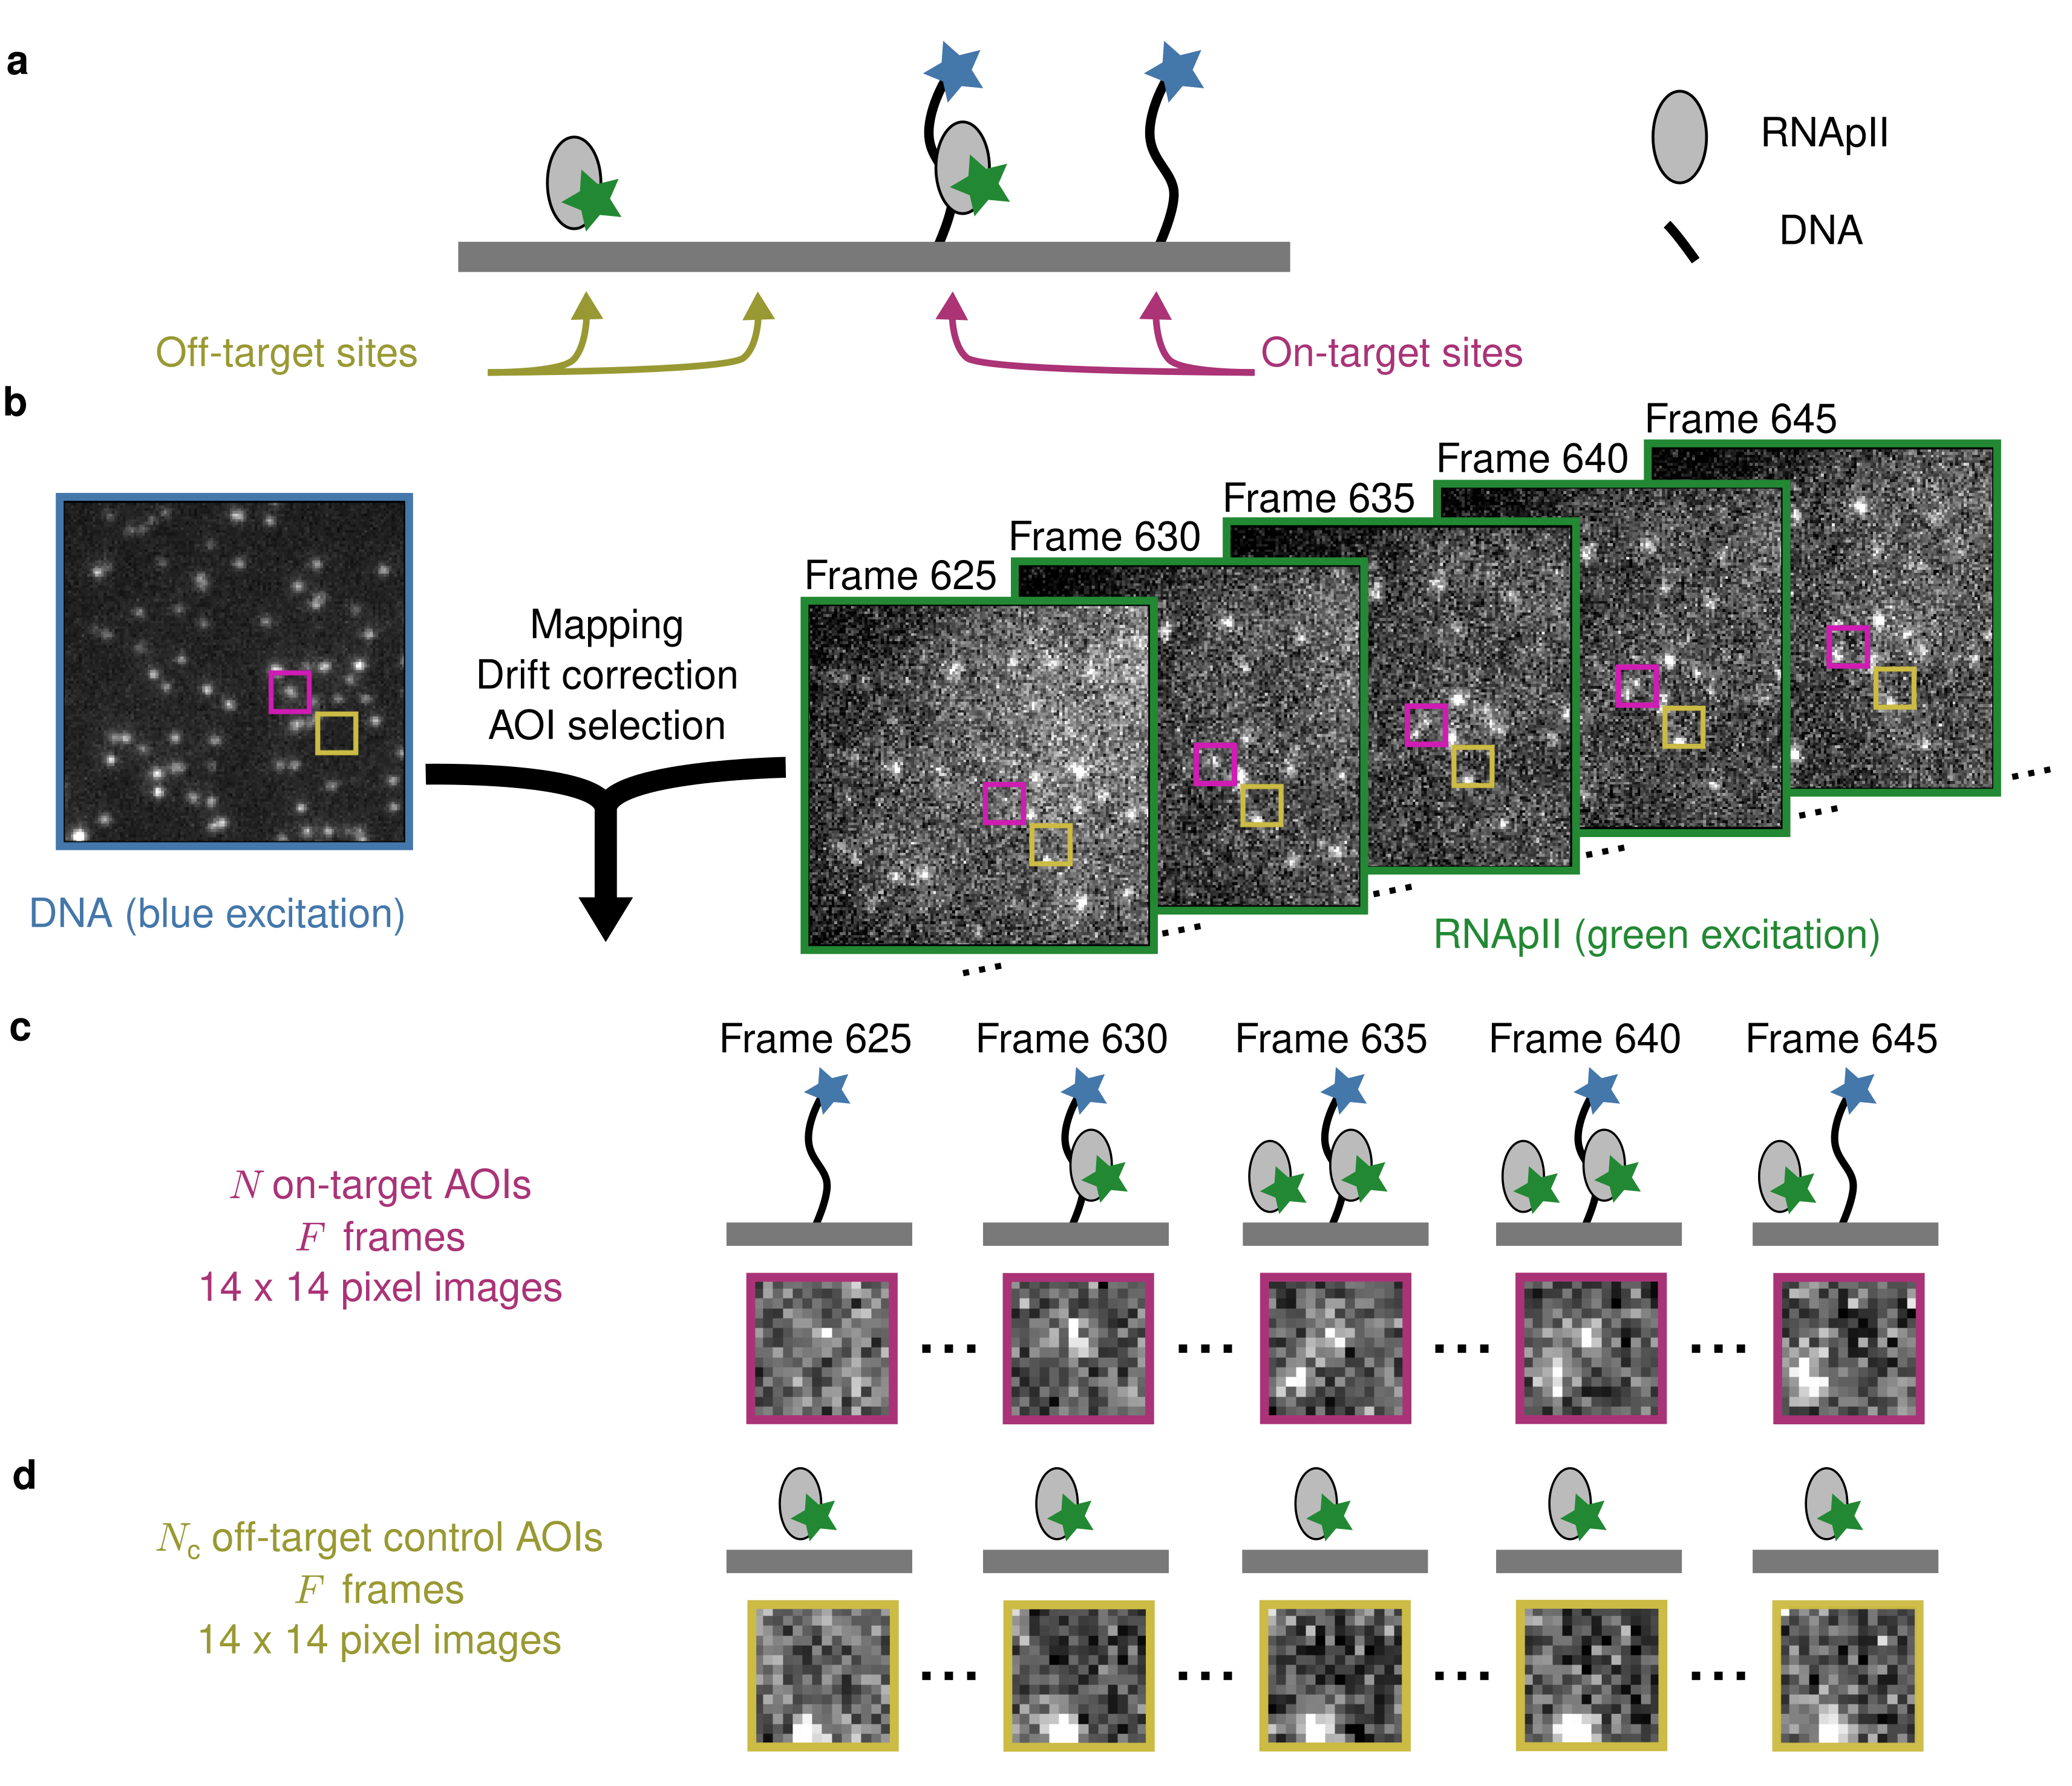
\includegraphics[width=\textwidth]{figures/figure1/figure1.png}
\caption{\textbf{Example CoSMoS experiment.} Rpb1\textsuperscript{SNAP549} data set (Extended Data Table 1). \textbf{a}, Experiment schematic. DNA target molecules labeled with a blue-excited fluorescent dye (blue star) are tethered to the microscope slide surface. RNA polymerase II (RNApII) binder molecules labeled with a green-excited dye (green star) are present in solution. \textbf{b}, Data collection and preprocessing. After collecting a single image with blue excitation to identify the location of the DNA molecules, a time sequence of RNApII images were collected with green excitation.  Preprocessing of the images includes mapping of the corresponding points in target and binder channels, drift correction, and identification of two sets of areas of interest (AOIs).  One set corresponds to locations of target molecules (e.g., purple square); the other corresponds to locations where no target is present (e.g., yellow square). \textbf{c}, On-target data. Data are time sequences of $14 \times 14$ pixel AOI images centered at each target molecule. Frames show on-target (e.g., frame 630) and off-target (e.g., frame 645) binding of RNApII molecules. \textbf{d}, Off-target control data. Control data consists of images collected from randomly selected sites at which no target molecule is present. }
\label{fig:cosmos_experiment}
\end{figure}

% figure 2
\begin{figure}[h]
\centering
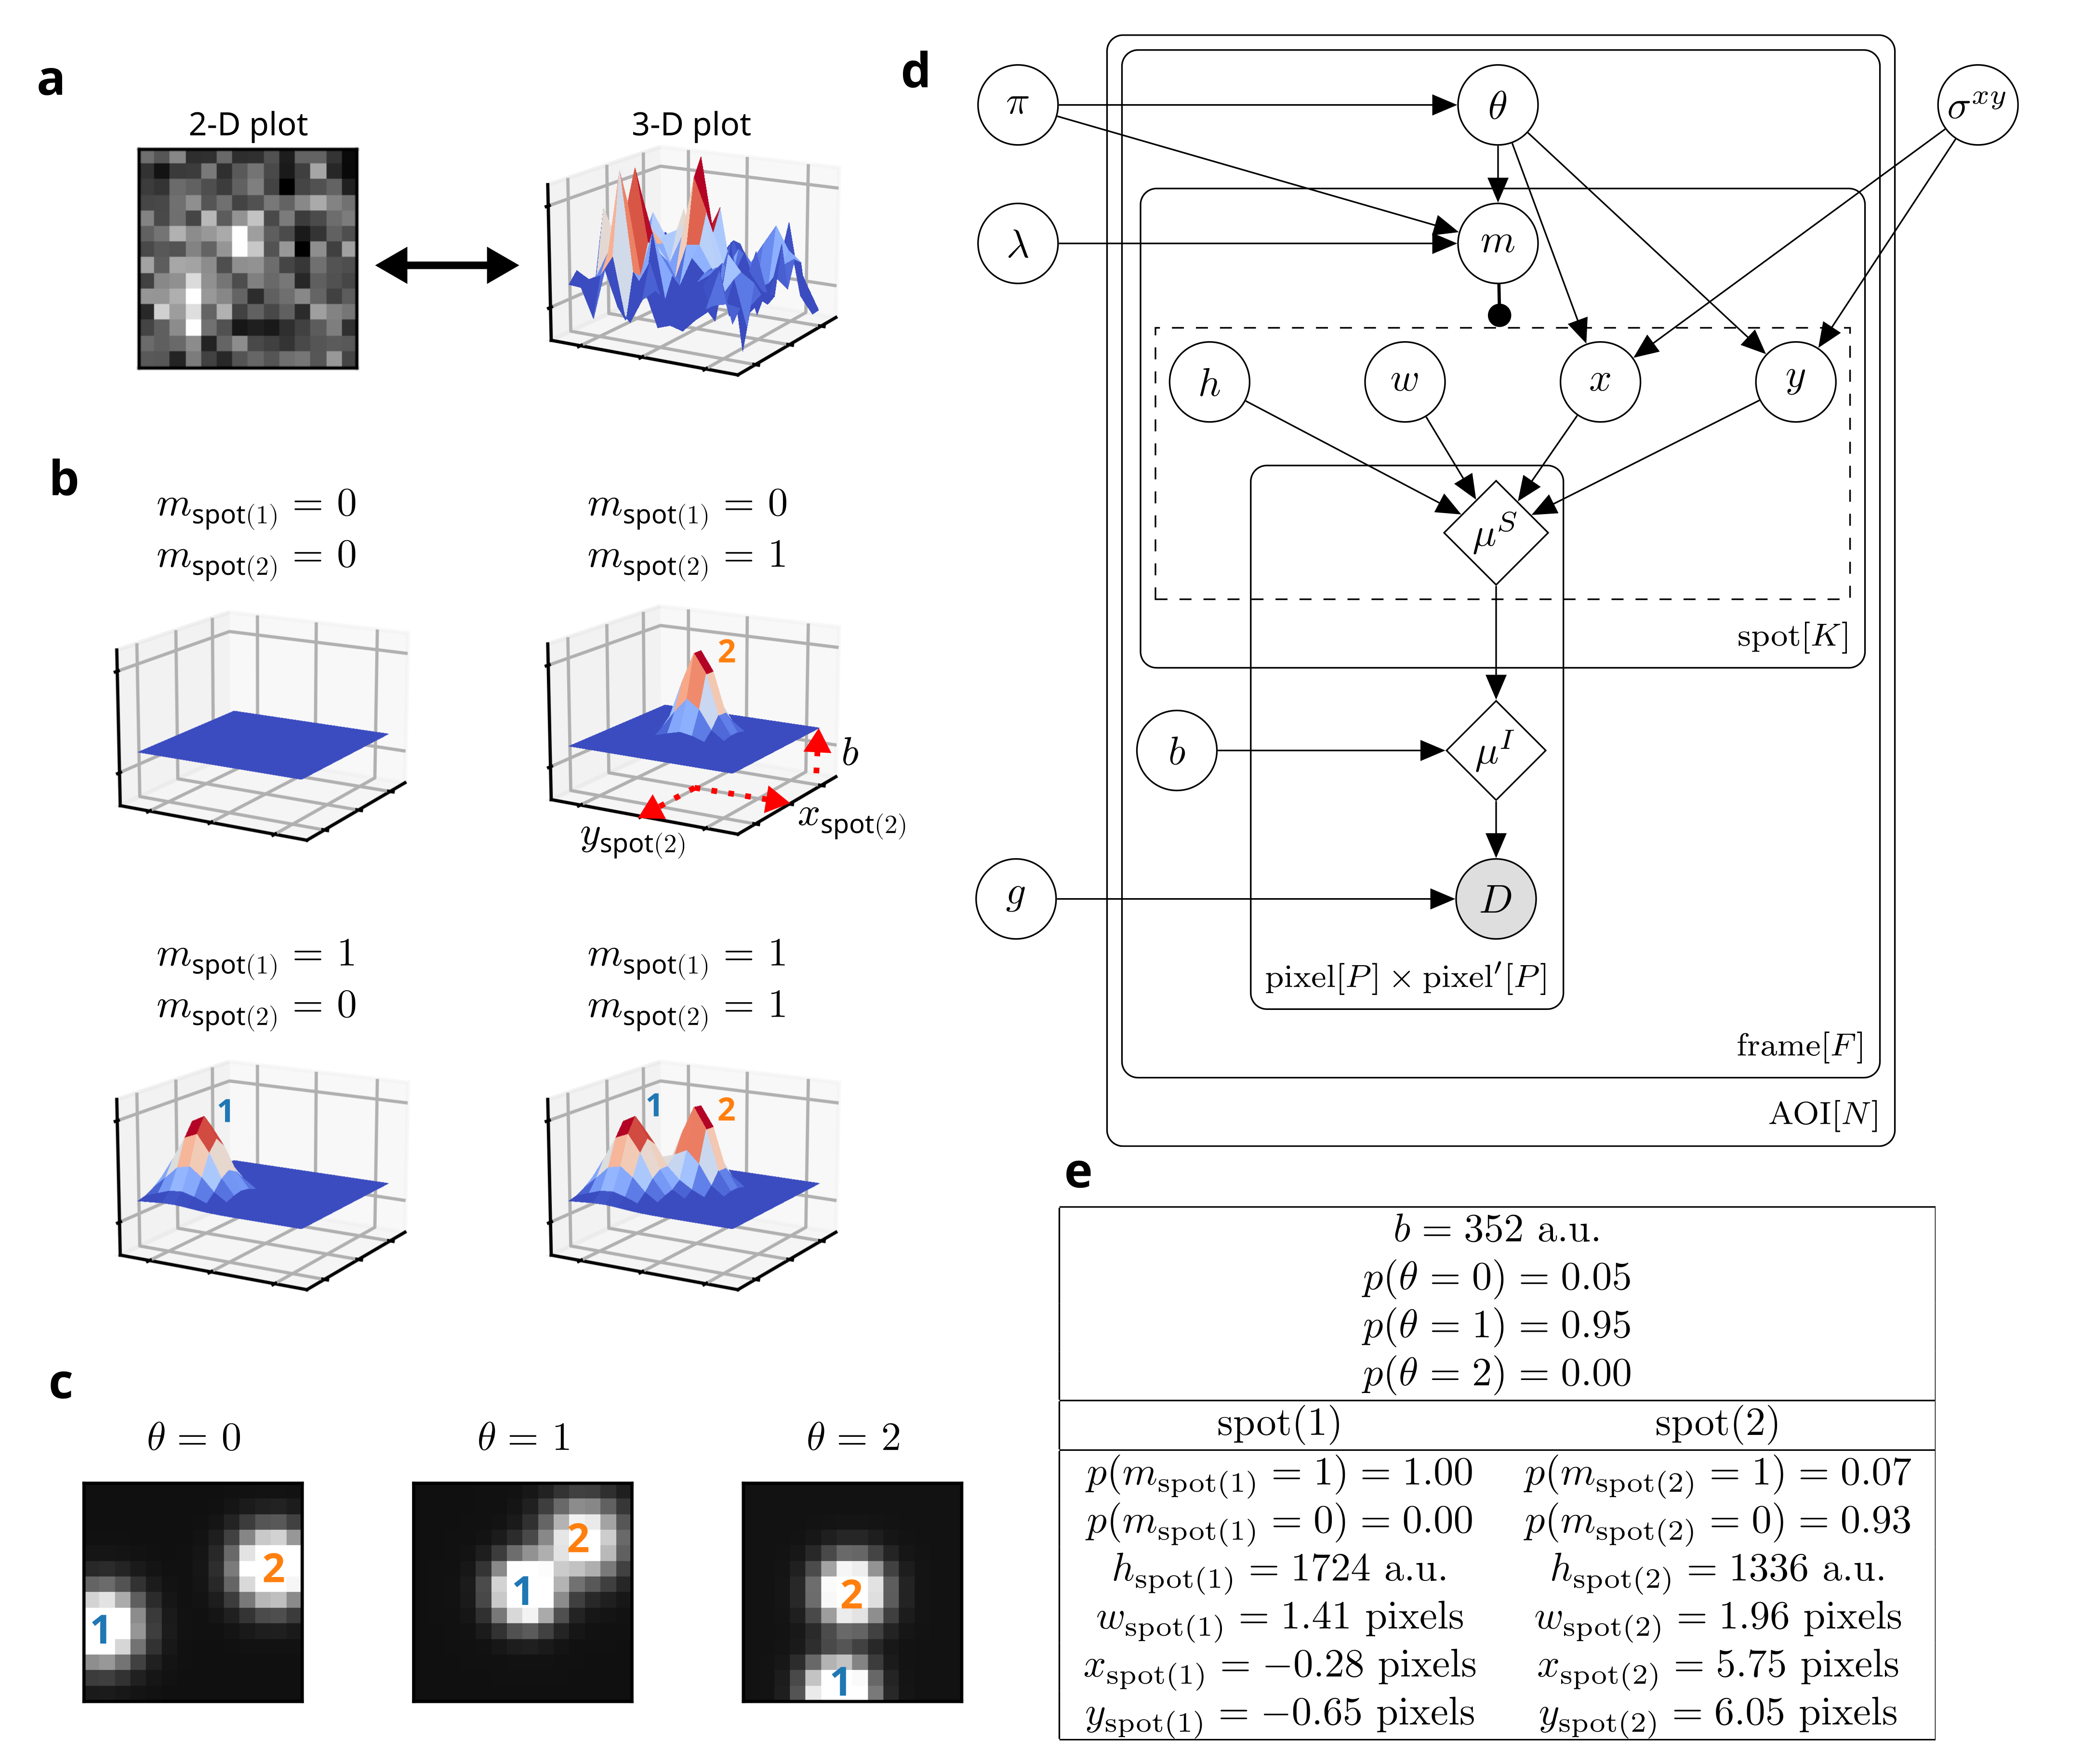
\includegraphics[width=\textwidth]{figures/figure2/figure2.png}
\label{fig:tapqir_model}
\caption{\textbf{Depiction of the probabilistic image model and model parameters.} \textbf{a}, Example AOI image from the Rpb1\textsuperscript{SNAP549} experimental data set. The image is a matrix (AOI) of $14 \times 14$ pixel intensities which is shown here as both a 2-D grayscale image and as a 3-D intensity plot. The image contains two spots, one is centered at target location (image center) and the other is located off-target. \textbf{b}, Examples of four idealized noise-free image representations ($\mu^I$). Image representations consist of zero, one, or two idealized spots ($\mu^S$) superimposed on a constant background ($b$). Each fluorescent spot is represented as a 2-D Gaussian parameterized by integrated intensity ($h$), width ($w$), and position ($x$, $y$). The presence of spots is encoded in the binary spot existence indicator $m$. \textbf{c}, Simulated idealized images illustrating different values of the target-specific spot index parameter $\theta$. $\theta = 0$ corresponds to a case when no specifically bound molecule is present; $\theta = 1$ or 2 corresponds to the cases in which the specifically bound molecule is spot 1 or 2, respectively. \textbf{d}, Condensed graphical representation of the probabilistic model. Model parameters are depicted as circles and deterministic functions as diamonds. Observed image ($D$) is represented by a shaded circle. Related nodes are connected by edges, with an arrow pointing towards the dependent node (e.g., the shape of each 2-D Gaussian spot $\mu^S$ depends on spot parameters $h$, $w$, $x$, and $y$). The dashed box represents activation of spot parameters based on the spot existence indicator $m$. Plates (rounded rectangles) contain entities that are repeated for the number of instances displayed at the bottom-right corner: number of AOIs ($N$), frame count ($F$), and/or maximum number of spots in a single image ($K=2$). Parameters outside of the plates are global quantities that apply to all frames of all AOIs. A more complete version of the graphical model specifying the relevant probability distributions is given in Extended Data Fig. 1a. \textbf{e}, Table of mean parameter values inferred from applying model (\textbf{d}) to the full dataset containing the image in (\textbf{a}). Image models in (\textbf{b}) correspond to parameters shown. }
\end{figure}

% figure 3
\begin{figure}[h]
\centering
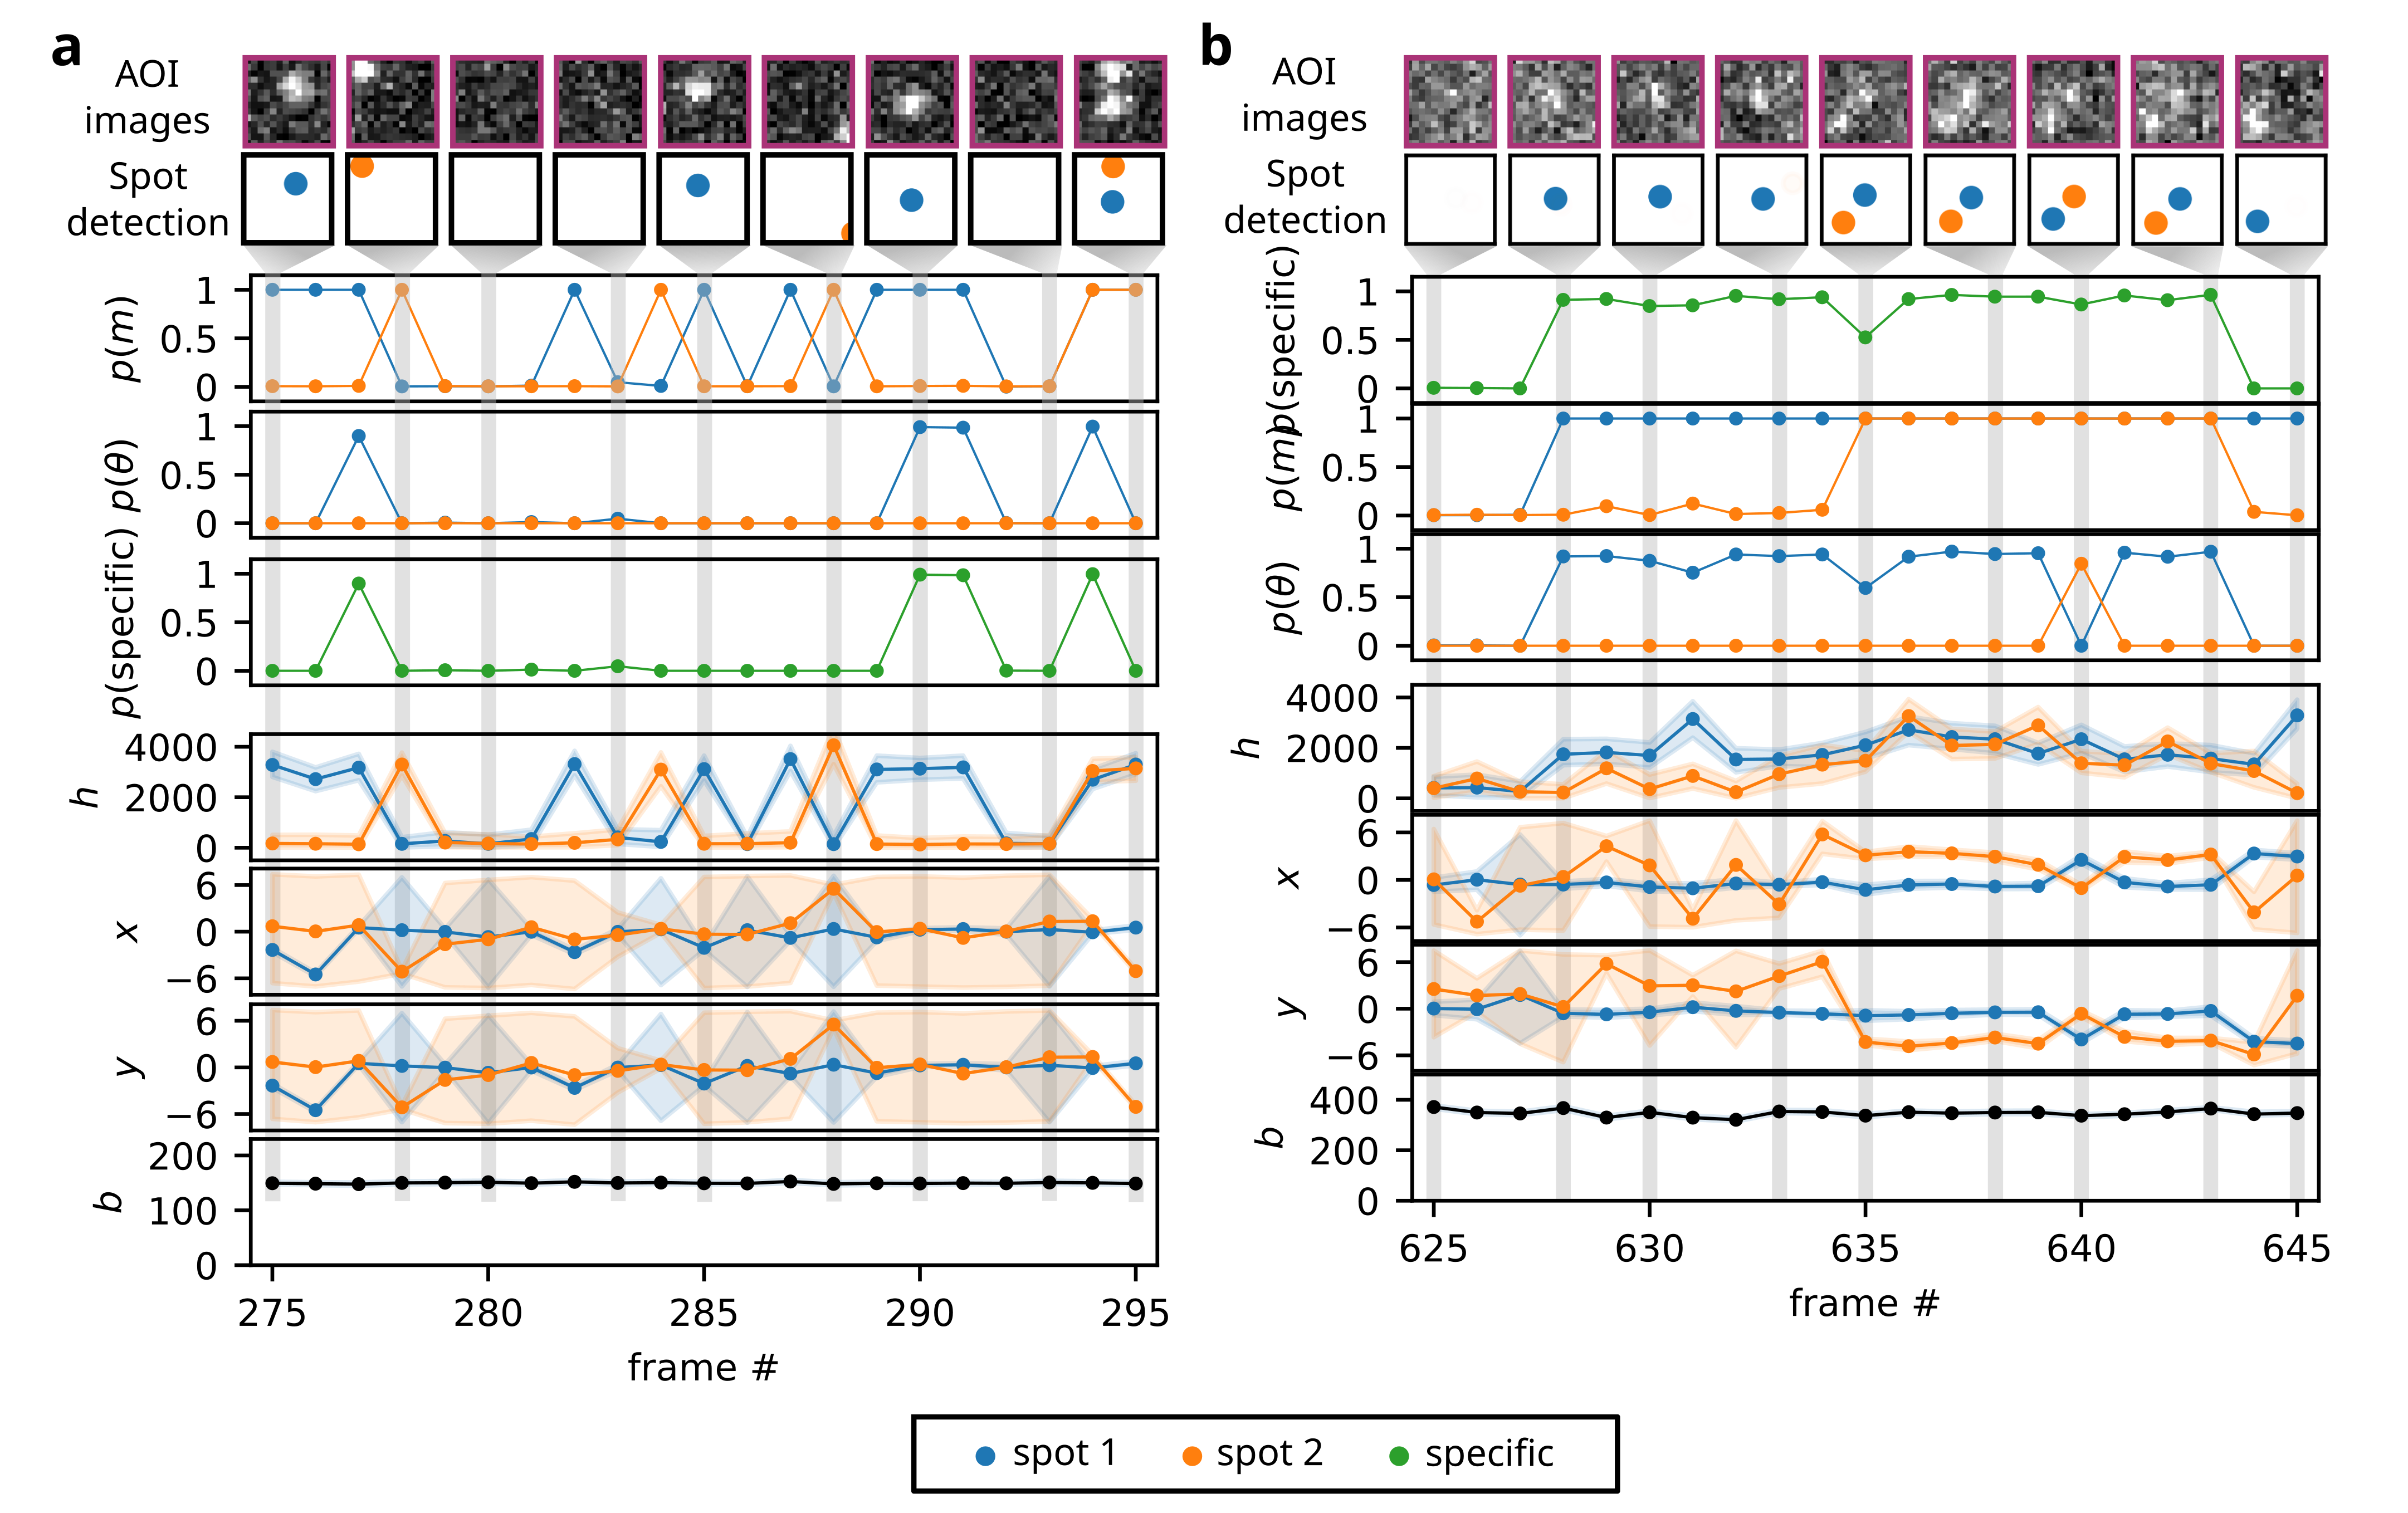
\includegraphics[width=\textwidth]{figures/figure3/figure3.png}
\caption{\textbf{Tapqir analysis and inferred model parameters.} \textbf{a},\textbf{b}, Tapqir was applied to simulated data (lamda0.5 parameter set in Supplementary Data 1) (\textbf{a}) and to experimental data (Rpb1\textsuperscript{SNAP549} in Extended Data Table 1) (\textbf{b}). (\textbf{a}) and (\textbf{b}) each show a short extract from a single target location in the corresponding data set. The first row shows AOI images for the subset of frames indicated by gray shaded stripes in the plots. The second row shows the locations of spots determined by Tapqir. Only data for spots with a spot probability $p(m=1) > 0.5$ are shown. Spots predicted to be target-specific ($p(\theta=k)>0.5$ for spot $k$) are shown as filled circles. The graphs show the probability of there being any target-specific spot in a frame ($p(\mathsf{specific})$; green), spot intensity ($h$), location ($x$, $y$) of spot 1 (blue) and spot 2 (orange), and AOI background intensity ($b$). Error bars: 95\% CI (credible interval).  }
\label{fig:tapqir_analysis}
\end{figure}

% figure 4
\begin{figure}[h]
\centering
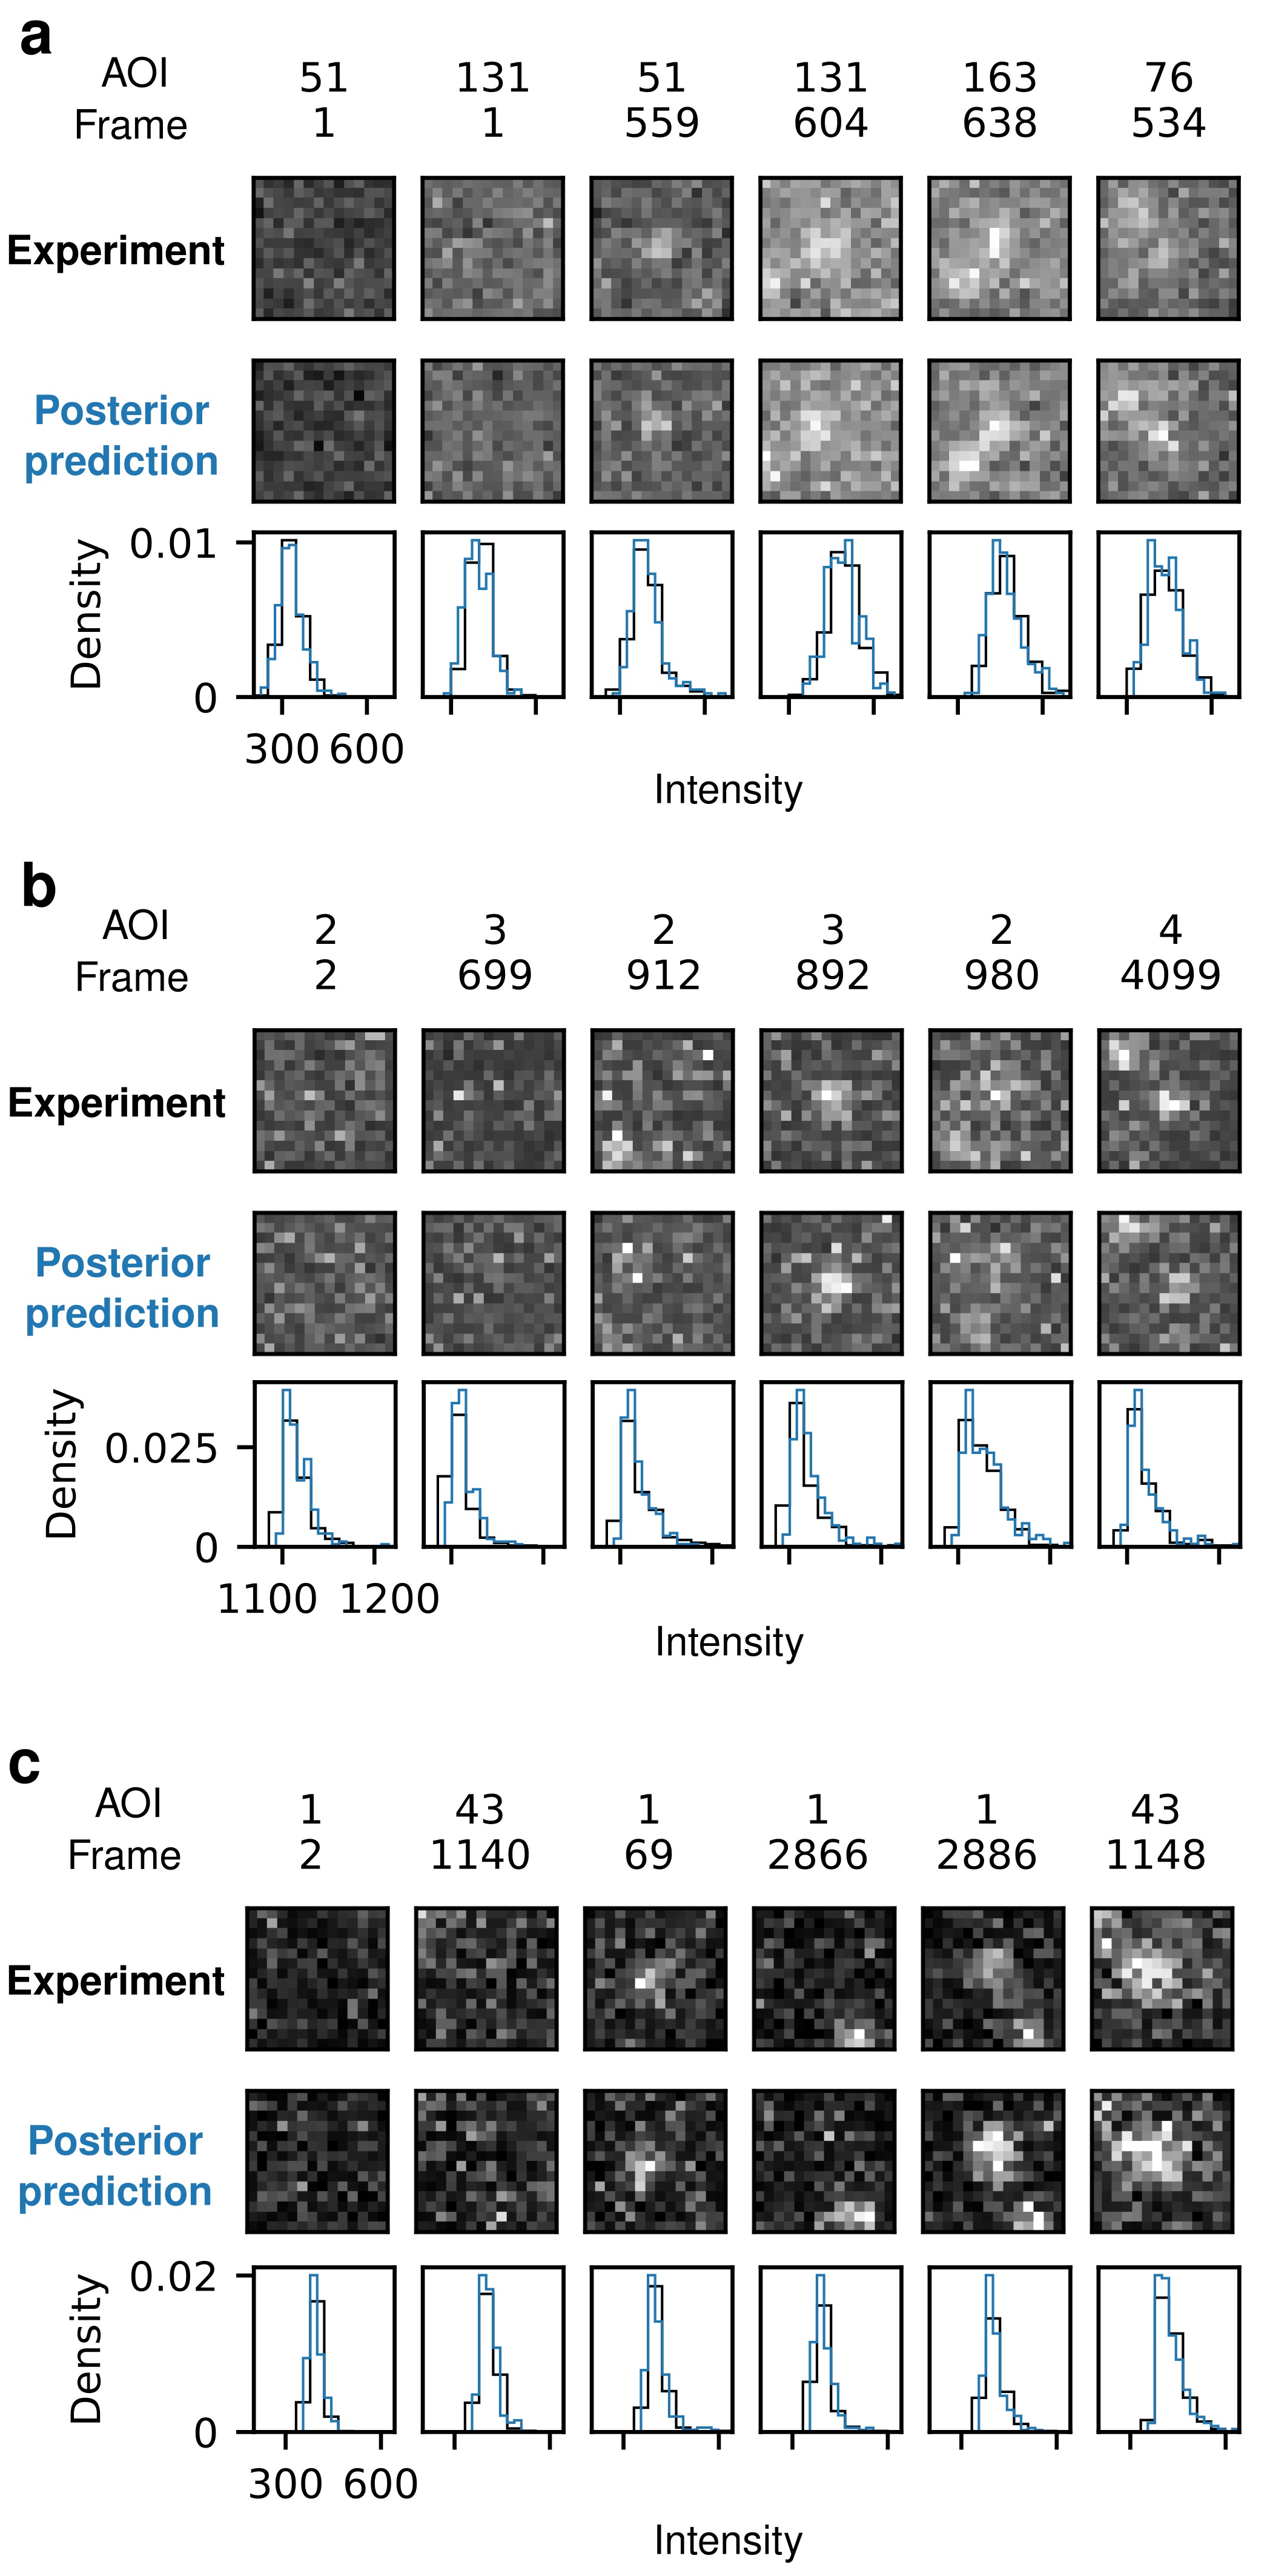
\includegraphics[width=0.5\textwidth]{figures/figure4/figure4.png}
\caption{\textbf{Reproduction of experimental data by posterior predictive sampling.} Example frames are shown from datasets Rpb1\textsuperscript{SNAP549}-DNA\textsuperscript{488} (\textbf{a}: $\mathrm{SNR}=1.61$), $\sigma^{54}$RNAPCy3-597P255 (\textbf{b}: $\mathrm{SNR}=3.38$), $\sigma^{54}$RNAPCy3-598P2993 (\textbf{c}: $\mathrm{SNR}=5.24$), and GreB (\textbf{d}: $\mathrm{SNR}=4.84$) in Extended Data Table 1. In each panel the top row shows AOI images selected from the experimental data and middle row shows corresponding images simulated by sampling from the posterior distributions. The bottom row shows pixel intensity distributions from the experimental and posterior prediction images shown. }
\label{fig:posterior_samples}
\end{figure}

% figure 5
\begin{figure}[h]
\centering
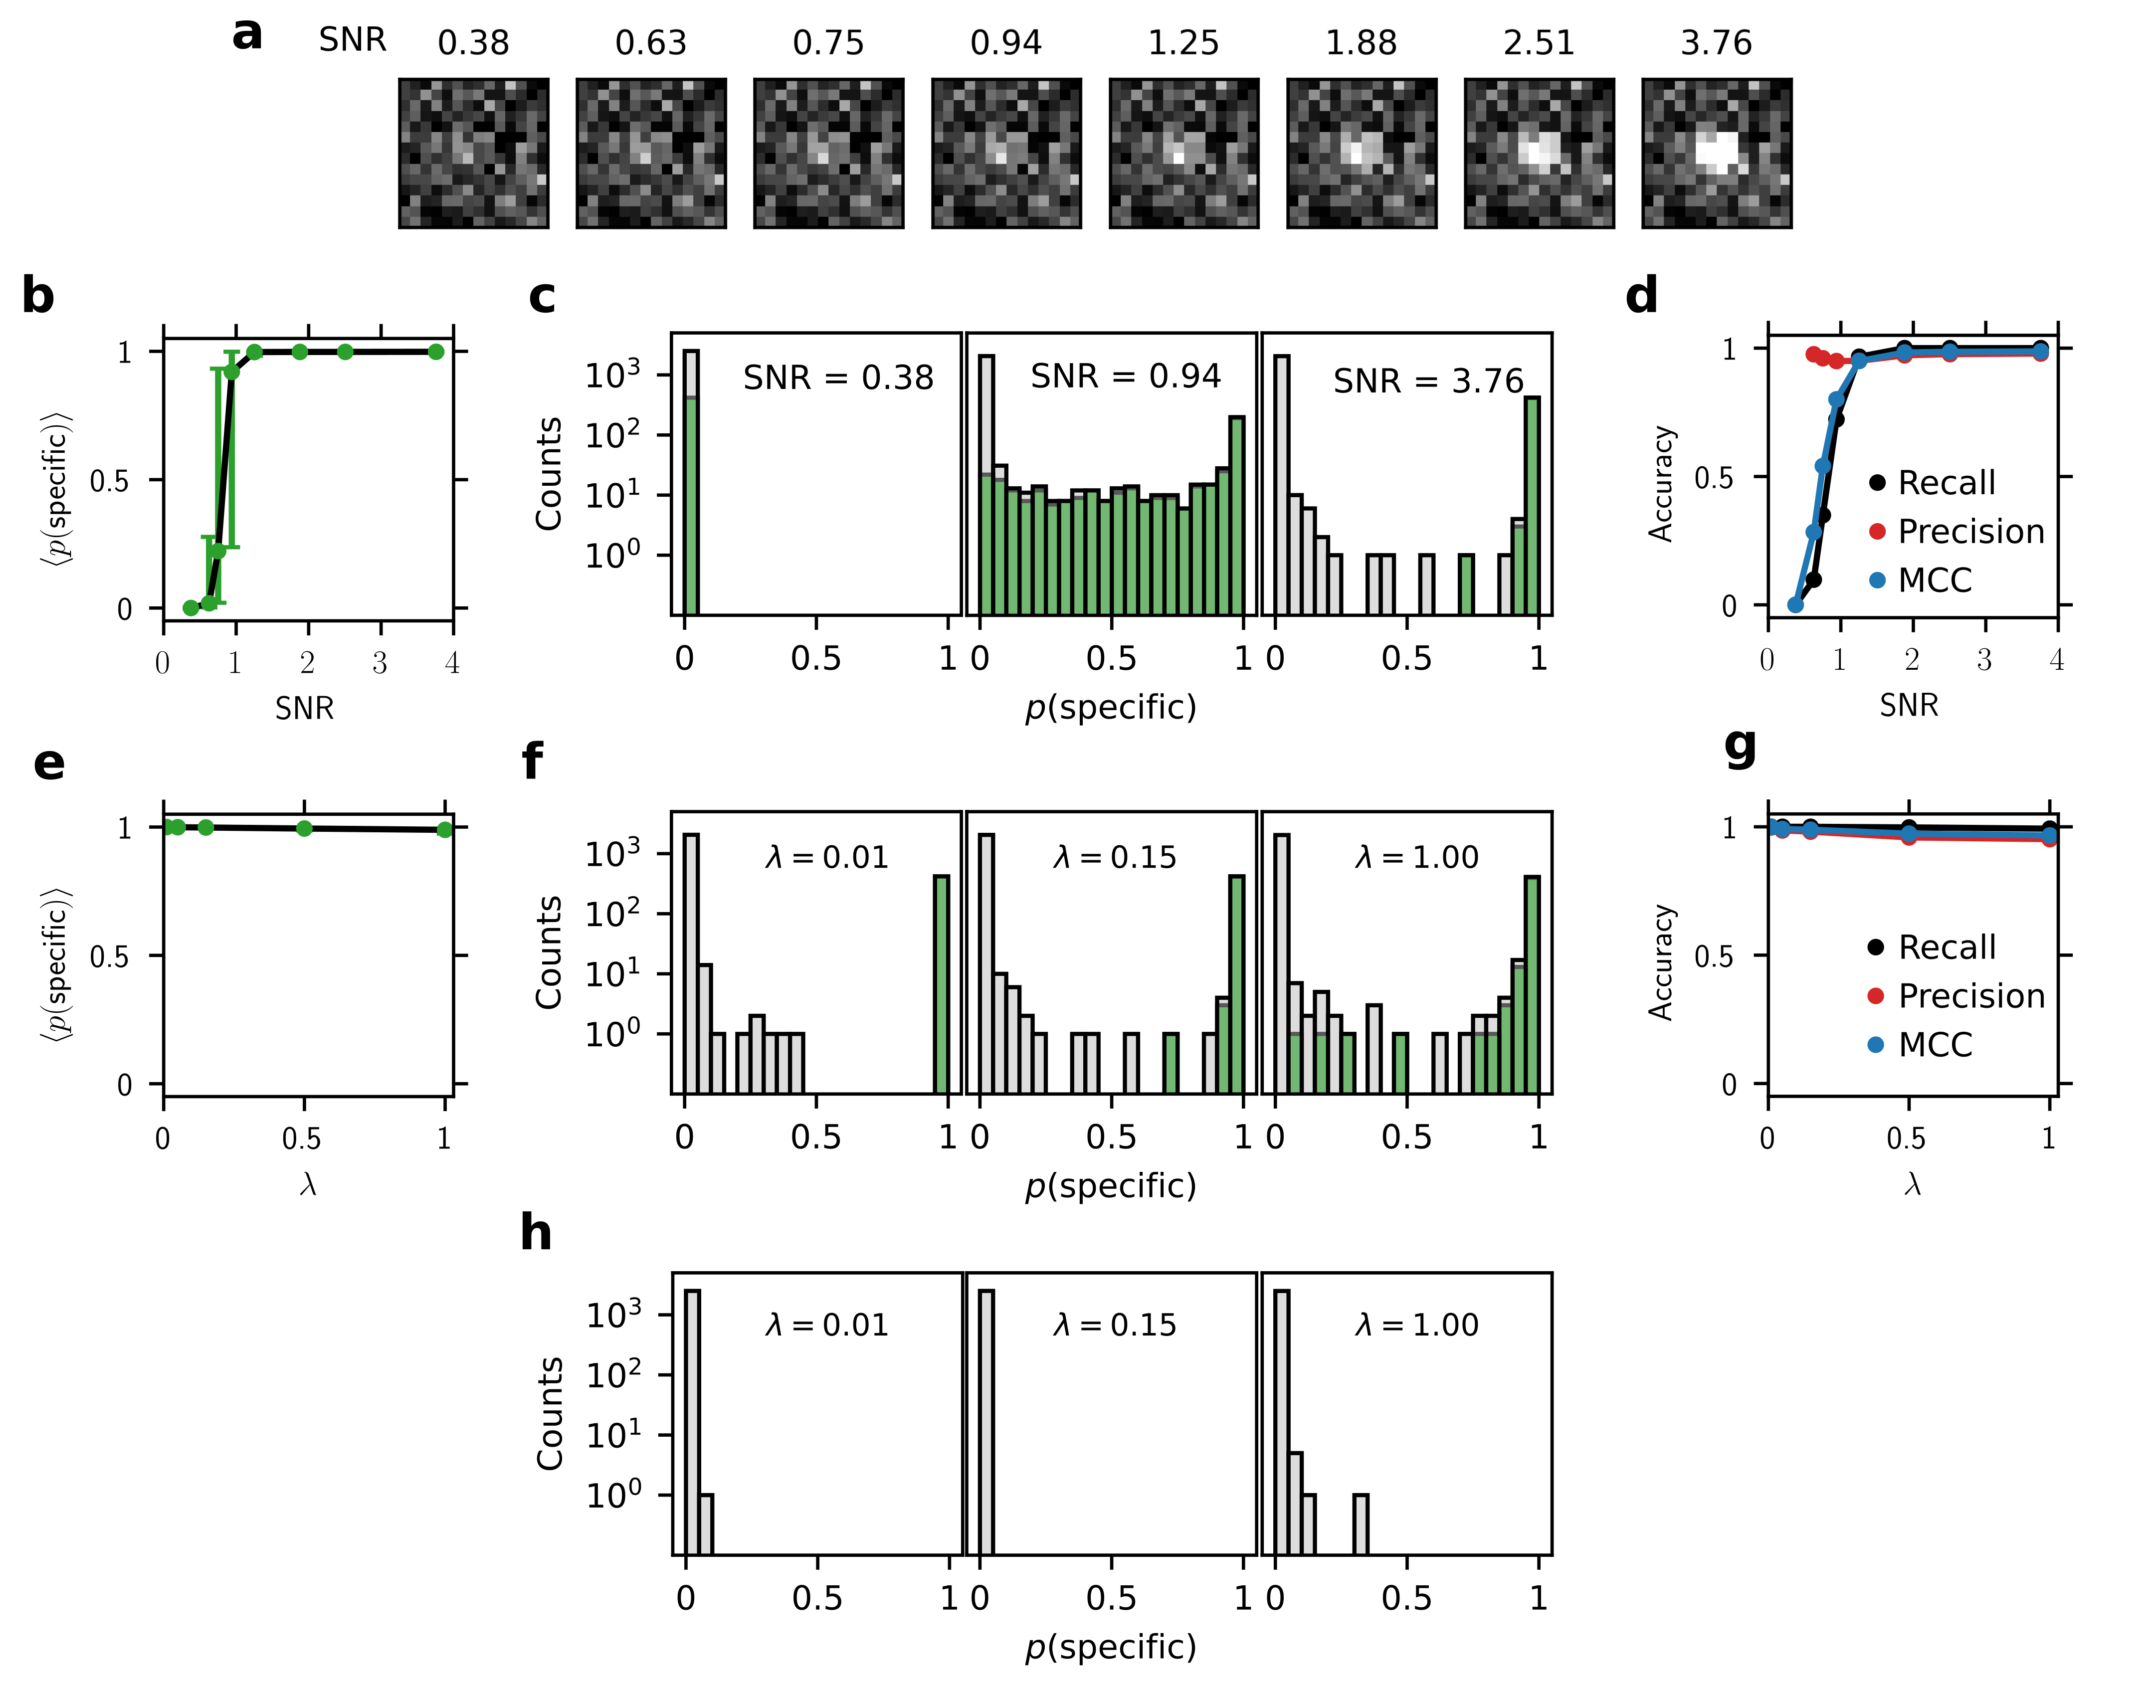
\includegraphics[width=1\textwidth]{figures/figure5/figure5.png}
\caption{\textbf{Tapqir performance on simulated data with different SNRs or different non-specific binding rates.} \textbf{a-d}, Analysis of simulated data over a range of SNR. SNR was varied in the simulations by changing spot intensity  $h$ while keeping other parameters constant (Supplementary Data 3). \textbf{a}, Example images showing the appearance of the same target-specific spot simulated with increasing SNR.   \textbf{b}, Mean of Tapqir-calculated target-specific spot probability $p(\mathsf{specific})$ (with 95\% high-density region) for the subset of images where target-specific spots  are known to be present. \textbf{c}, Histograms of $p(\mathsf{specific})$ for selected simulations with SNR indicated. Data are shown as stacked bars for images known to have (green, 15\%) or not have (gray, 85\%) target-specific spots.  Count is zero for bins where bars are not shown. \textbf{d}, Accuracy of Tapqir image classification with respect to presence/absence of a target-specific spot. Accuracy was assessed by MCC, recall, and precision (see Text and Methods). \textbf{e-g}, Same as in (\textbf{b-d}) but for the data simulated over a range of non-specific binding rates $\lambda$ at fixed SNR = 3.76 (Supplementary Data 1). \textbf{h}, Same as in (\textbf{c}) but for the data simulated over a range of non-specific binding rates $\lambda$ with no target-specific binding ($\pi = 0$) (Supplementary Data 4).}
\label{fig:tapqir_performance}
\end{figure}

% figure 6
\begin{figure}[h]
\centering
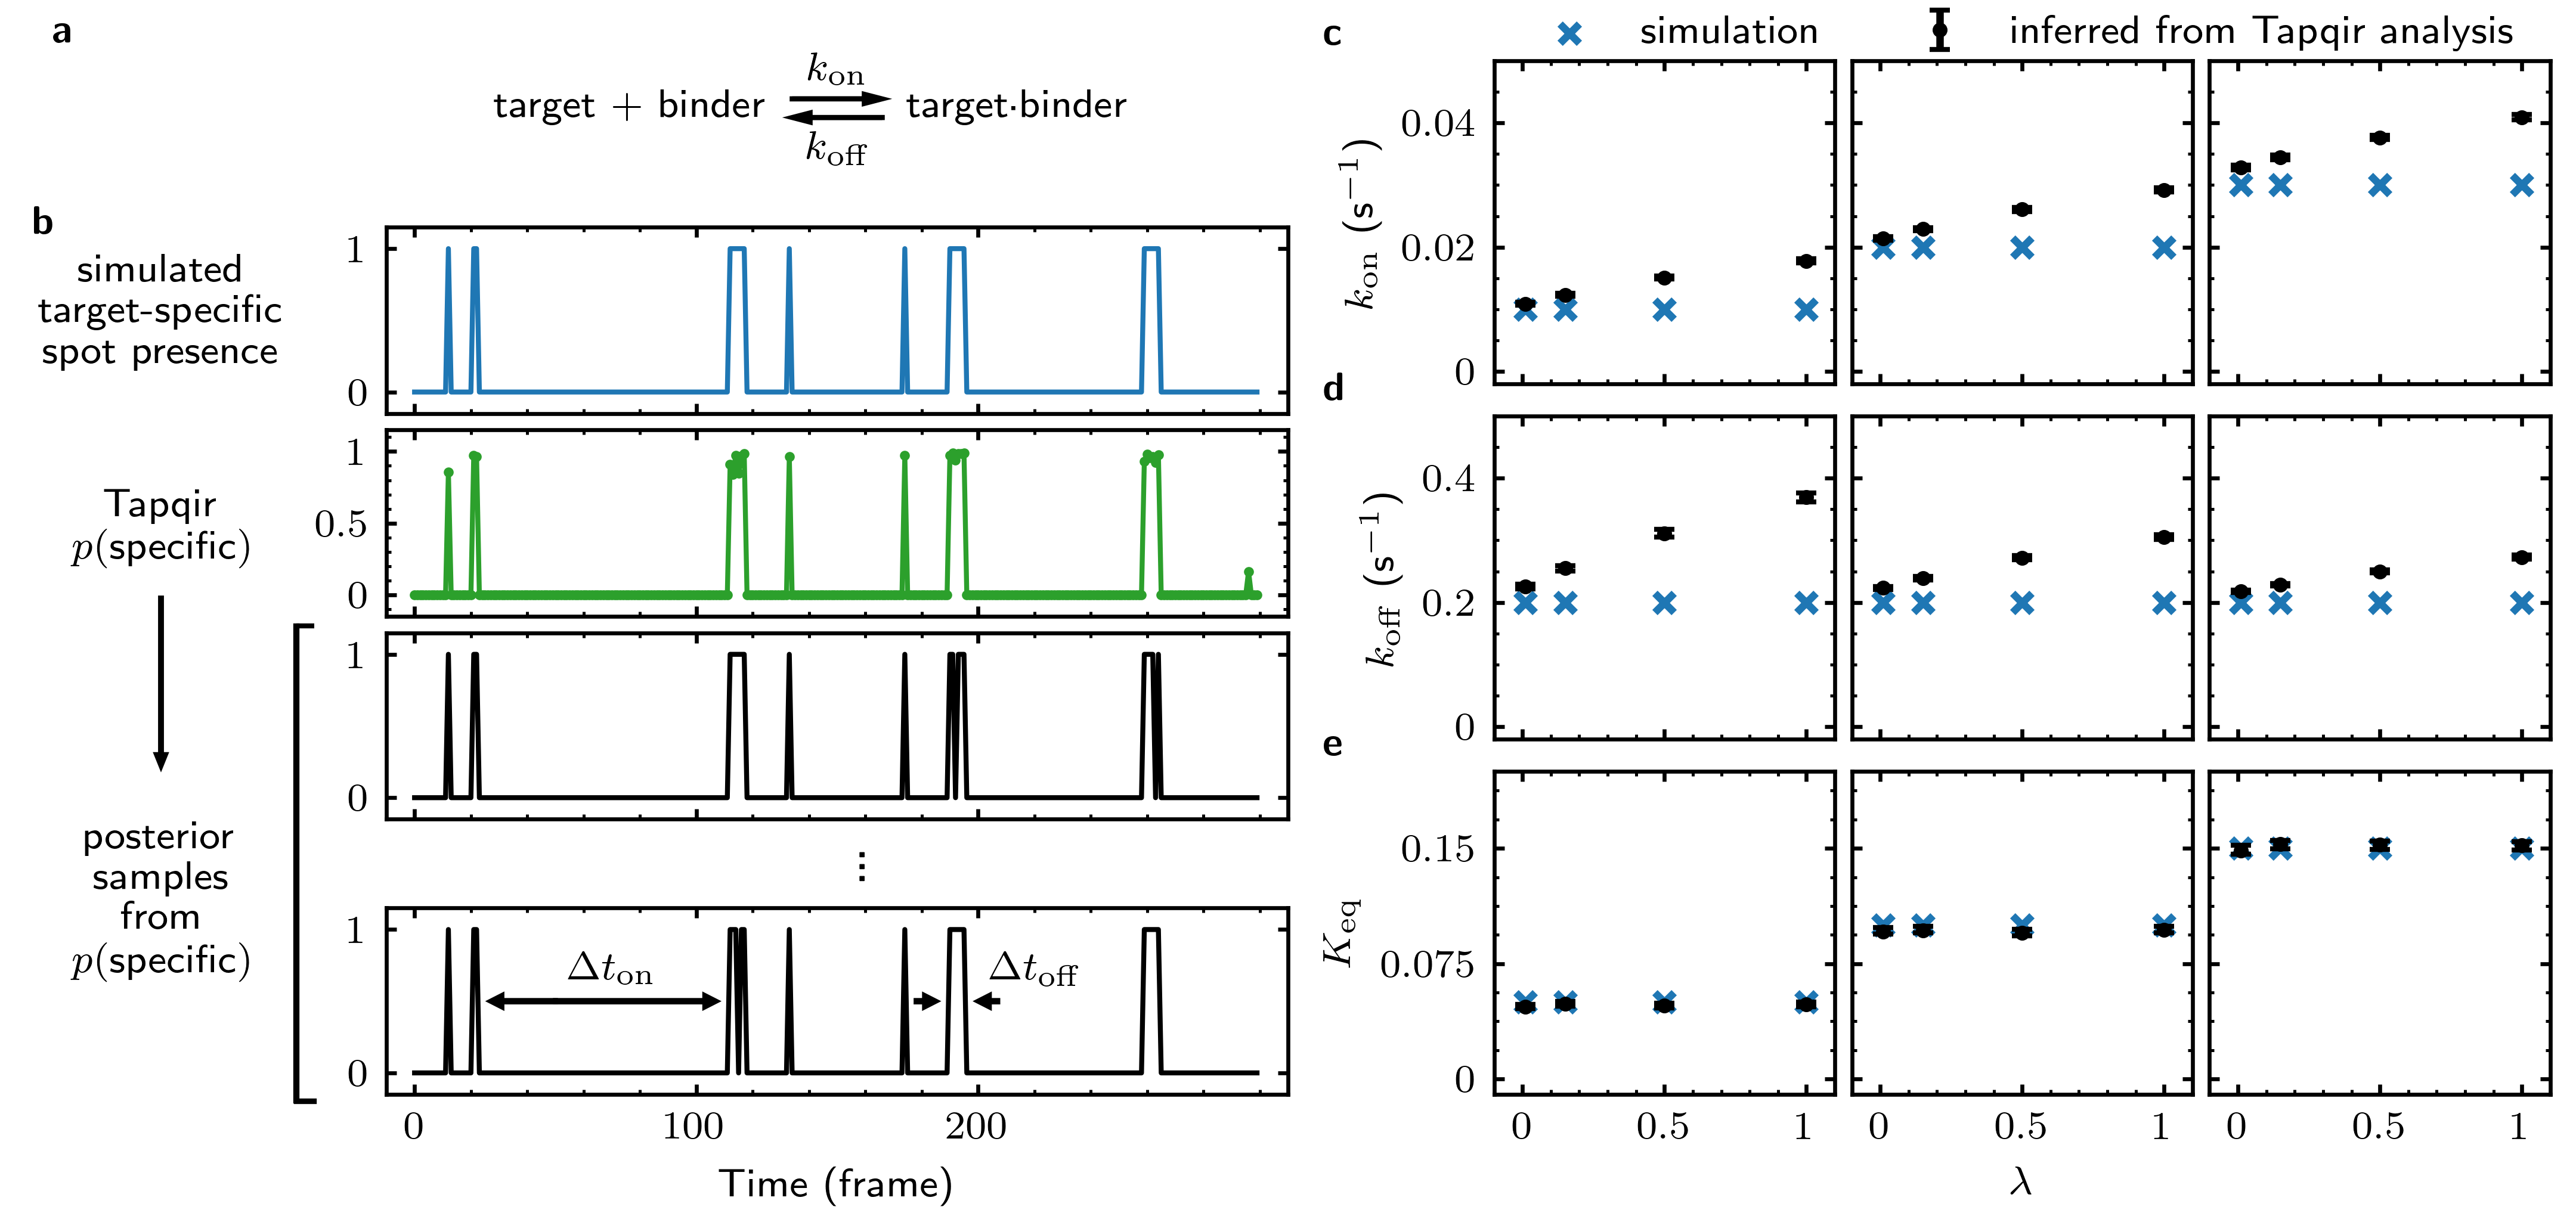
\includegraphics[width=183mm]{figures/figure6.png}
\caption{\textbf{Tapqir analysis of association/dissociation kinetics and thermodynamics.} \textbf{a} Chemical scheme for a one-step association/dissociation reaction at equilibrium with apparent first-order binding and dissociation rate constants $k_{\mathrm{on}}$ and $k_{\mathrm{off}}$, respectively. \textbf{b}, A simulation of the reaction in (\textbf{a}) and scheme for kinetic analysis with Tapqir. Simulation used $\mathrm{SNR} = 3.76$, $k_\mathrm{on} = 0.02$ s$^{-1}$, $k_\mathrm{off} = 0.2$ s$^{-1}$, and a high target-nonspecific binding frequency $\lambda = 1$ (Supplementary Data 5, dataset kon0.02lambda1). Full dataset consists of 100 AOI locations and 1000 frames each for on-target data and off-target control data. Shown is a short extract of on-target data from a single location in the simulation.  Plots show simulated presence/absence of the target-specific spot (purple) and Tapqir-calculated estimate of corresponding target-specific spot probability $p(\mathsf{specific})$ (green). One thousand binary traces (e.g., black records) were sampled from the $p(\mathsf{specific})$ posterior distribution and used to infer $k_\mathrm{on}$ and $k_\mathrm{off}$ using a two-state hidden Markov model (HMM) (see Methods). Each sample trace contains well-defined time intervals corresponding to target-specific spot presence and absence (e.g., $\Delta t_\mathrm{on}$ and $\Delta t_\mathrm{off}$). \textbf{c,d,e}, Kinetic and equilibrium constants from simulations (Supplementary Data 5) using a range of $k_\mathrm{on}$ values and  target-nonspecific spot frequencies $\lambda$, with constant $k_\mathrm{off} = 0.2$ s$^{-1}$. \textbf{c} Values of $k_{\mathrm{on}}$ used in simulations (blue) and mean values (and 95\% CIs, black) inferred by HMM analysis from the 1000 posterior samples. \textbf{d}, Same as (\textbf{c}) but for $k_{\mathrm{off}}$. \textbf{e},  Binding equilibrium constants $K_{\mathrm{eq}} = k_{\mathrm{on}} / k_{\mathrm{off}}$ used in simulation (blue) and inferred from Tapqir-calculated $\pi$ as $K_{\mathrm{eq}} = \pi / (1 - \pi)$ (black). }
\label{fig:kinetic_analysis}
\end{figure}
% do 2000 simulations
\clearpage
\pagebreak

% figure 7
\begin{figure}[h]
\centering
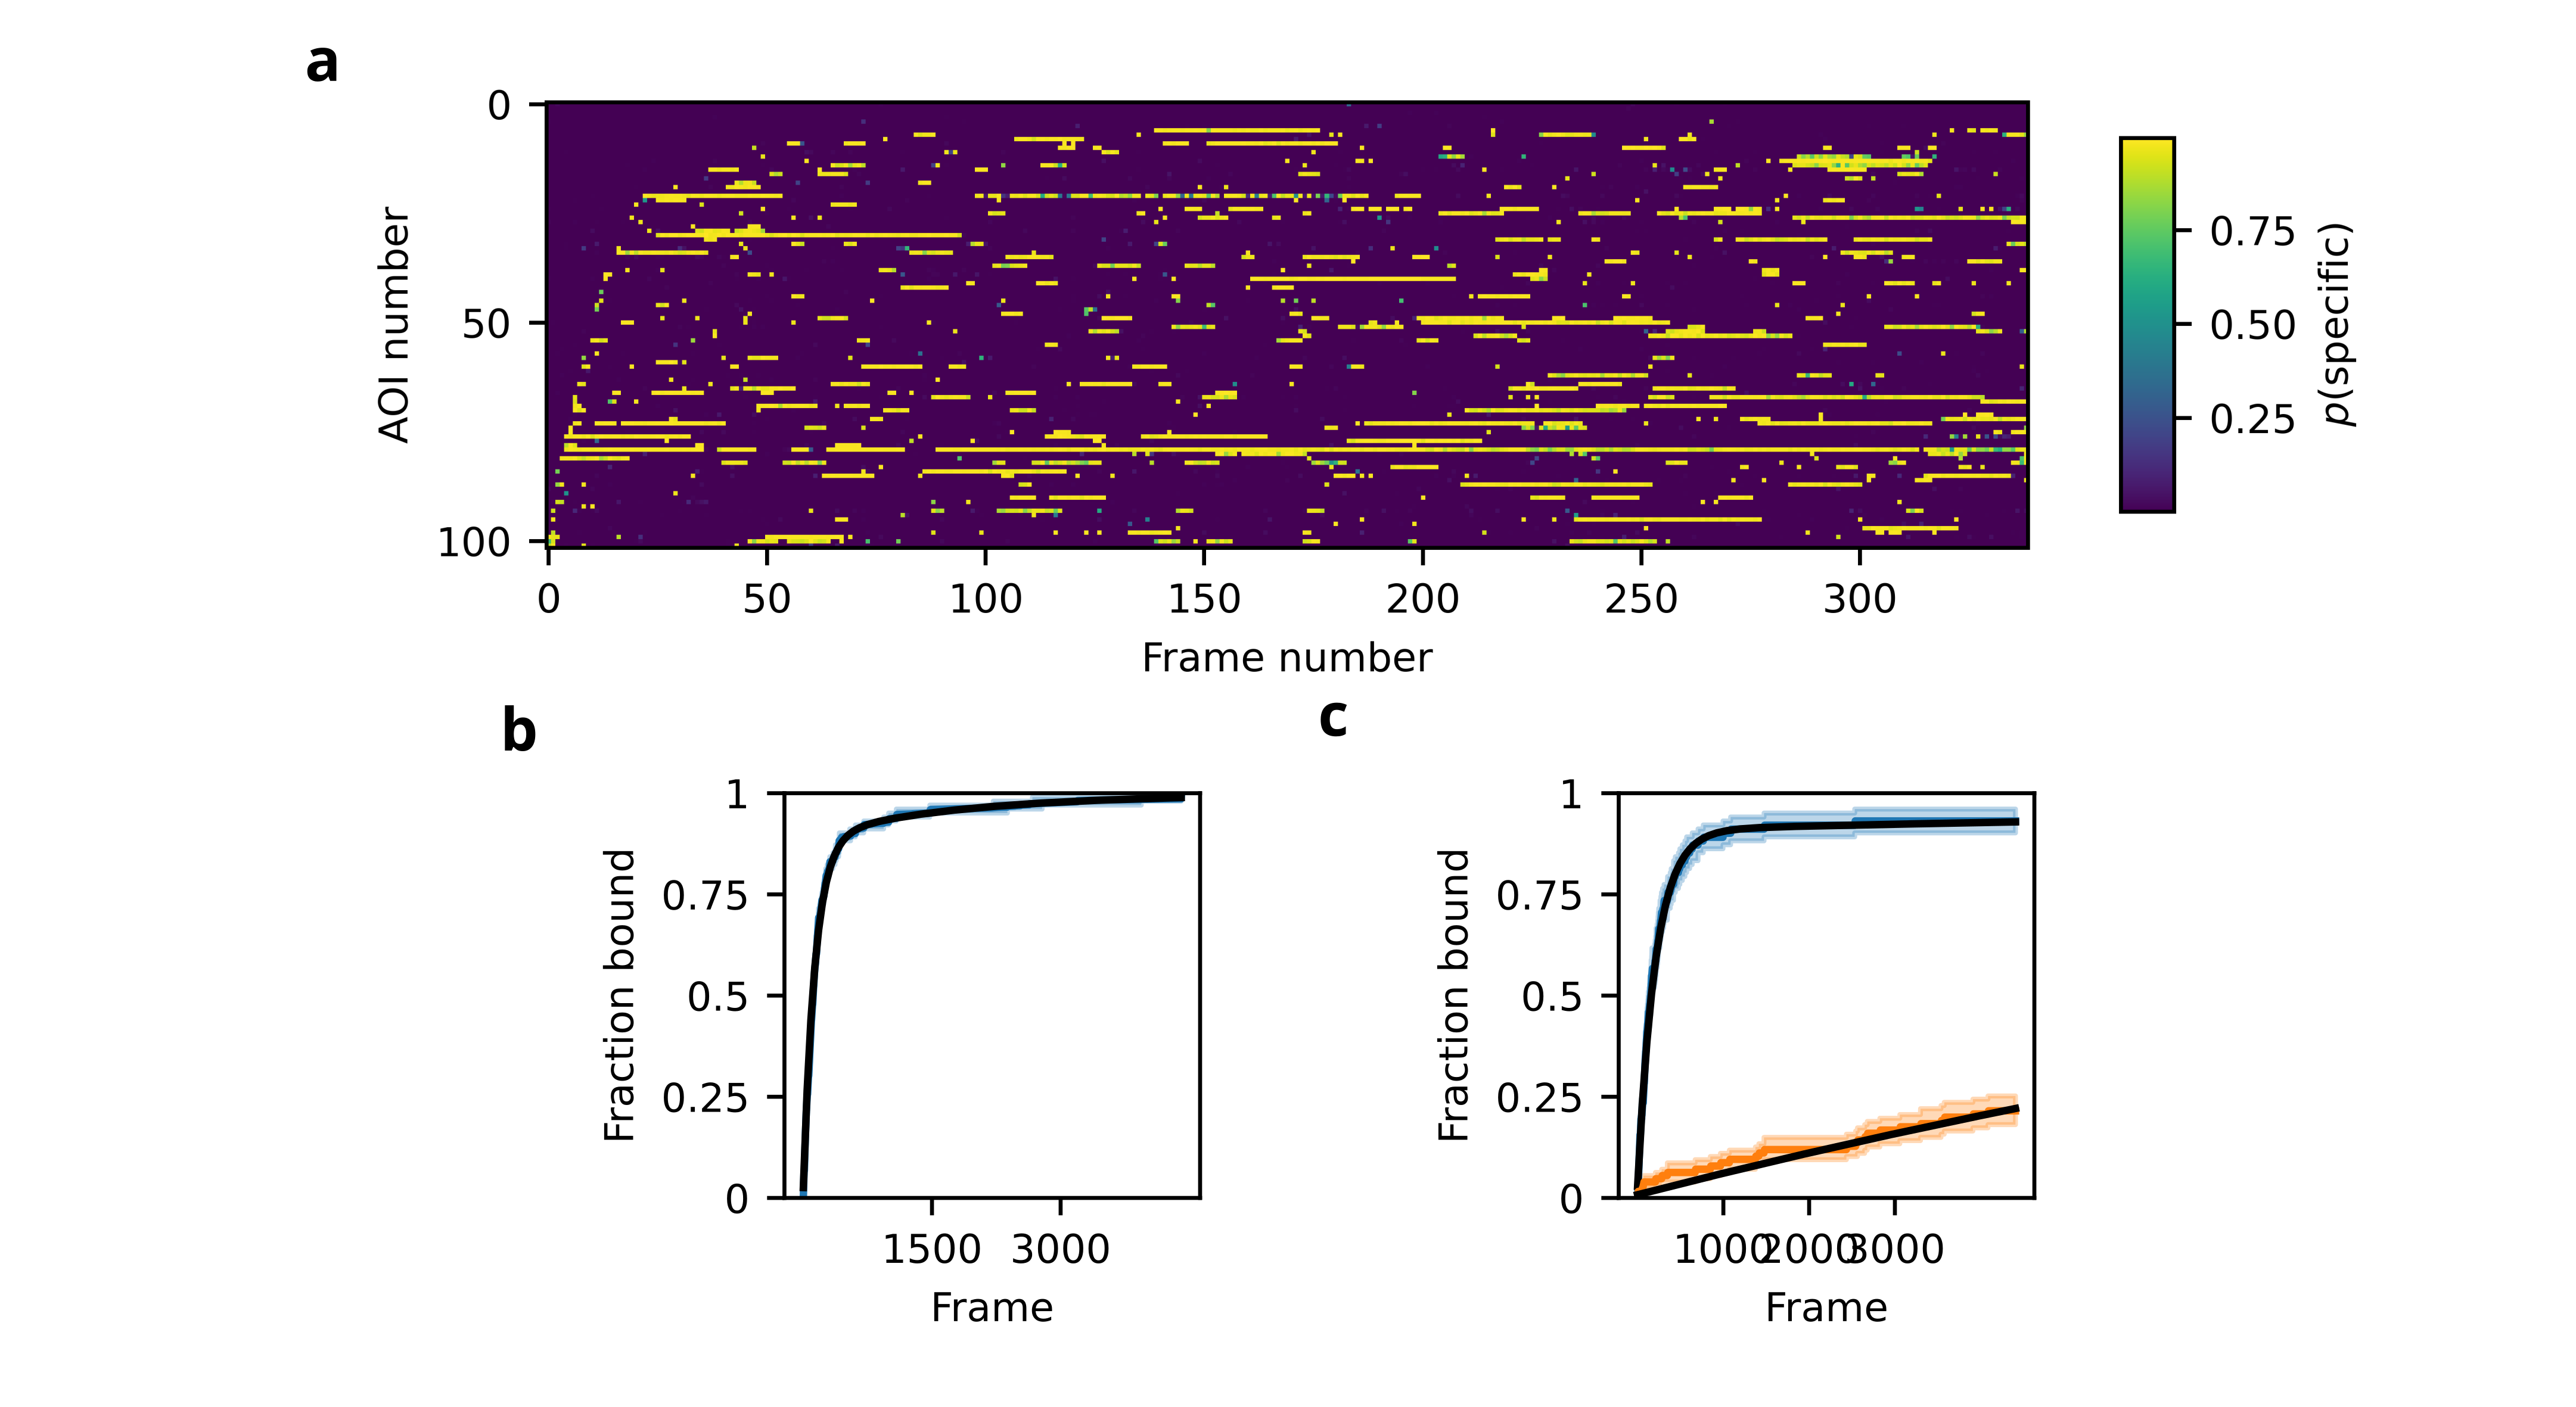
\includegraphics[width=\textwidth]{figures/figure7/figure7.png}
\caption{\textbf{Kinetic analysis of experimental data.} Data set: $\sigma^{54}$RNAPCy3-597P255 in Extended Data Table 1.  \textbf{a}, Probabilistic rastergram representation of Tapqir-calculated target-specific spot  probabilities $p(\mathsf{specific})$ (color scale). AOIs were ordered by decreasing times-to-first-binding. For clarity, only every 13\textsuperscript{th} frame is shown. \textbf{b,c}, Determining the association kinetic parameters [95\% CI] by  time-to-first-binding analysis using Tapqir (\textbf{b}) and an empirical spot-picker method \cite{Friedman2013-sf}(\textbf{c}).   Cumulative fraction of target sites that exhibited one or more binding events by the indicated frame number (blue) and fit curve (black) yielding best-fit values for $k_\mathrm{a}$, $k_\mathrm{ns}$, and $A_\mathrm{f}$. Shading indicates 95\% CI. Fitting protocol is different for the two methods; the spot-picker method fits both the target sites and off-target control data (orange) whereas Tapqir incorporates the control data in its $p(\mathsf{specific})$ calculation. \textbf{d}, Fit parameters.
}
\label{fig:experimental_data}
\end{figure}
% check CI - hdpi or pi?
%Tapqir (\textbf{b}: $k_\mathrm{a} = 5.59 \: [4.62, 6.62] \times 10^{-3}$ s$^{-1}$, $k_\mathrm{ns} = 5.9 \: [2.4, 10.5] \times 10^{-4}$ s$^{-1}$, $A_\mathrm{f} = 0.85 \: [0.77, 0.93]$) and an empirical spot-picker method (\textbf{c}: $k_\mathrm{a} = 4.78 \: [3.65, 6.20] \times 10^{-3}$ s$^{-1}$, $k_\mathrm{ns} = 5.5 \: [3.5, 7.7] \times 10^{-5}$ s$^{-1}$, $A_\mathrm{f} = 0.91 \: [0.84, 0.96]$) 